
\begin{figure}[h]
  \centering
  \begin{tabular}{ p{3.2cm} p{4.5cm} p{4.5cm} }
    \centering 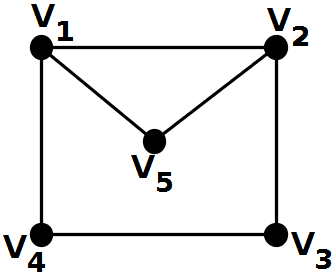
\includegraphics[width=3cm]{./img/envelope} & 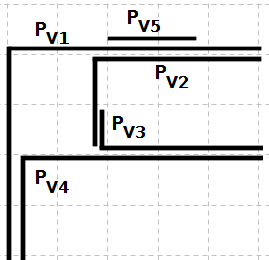
\includegraphics[width=4cm]{./img/envelopeHellyGradeTransparente} & 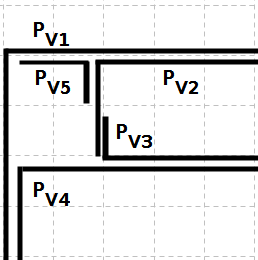
\includegraphics[width=4cm]{./img/envelopeNaoHellyGrade}
    \\
    \footnotesize \centering (a) A  graph with 5 vertices. & \footnotesize(b) A $B_1$-EPG representation that satisfies the Helly property. & \footnotesize (c) A $B_1$-EPG representation that does  not satisfy the Helly property.  \\

  \end{tabular}
\caption{A  graph with 5 vertices in (a) and some single bend representations: Helly in (b) and not Helly in (c).} \label{fig:envelopeRepresentacoes}
\end{figure}

%%%%%%%%%%%%%%%%%%%%%%%%%%%%%%%%%%%%%%%%%%%%%%%%%%%%%%%%%%%%%